\documentclass[a4paper,12pt]{article}
\usepackage{amsmath, amsthm, amsfonts, amssymb}
\usepackage{mathtools}
\usepackage{microtype}
\usepackage{geometry}
\usepackage{booktabs}
\usepackage{graphicx}
\usepackage{tikz}
\usepackage{caption}
\usepackage{subcaption}
\usepackage{xparse}
% \geometry{margin=1in}
\usepackage{minted}
\usepackage{enumitem}
\usepackage{comment}
\usepackage{hyperref}
\usepackage{placeins}
\usepackage{xcolor}
\hypersetup{ % this is just my personal choice, feel free to change things
    colorlinks,
    linkcolor={red!50!black},
    citecolor={blue!50!black},
    urlcolor={blue!80!black},
}


\colorlet{myred}{red!20}
\colorlet{myblue}{blue!20}
\colorlet{mypurple}{purple!40}
\colorlet{myorange}{orange!20}
\colorlet{myteal}{teal!35}

% Your existing style for exercises, copied from your code:
\newtheoremstyle{exerciseStyle}%
{}{}%
{\normalfont}%
{}%
{\bfseries}%
{}%
{ }%
{\thmname{#1}\thmnumber{ #2}} % The heading "Exercise 4.6", etc.

\theoremstyle{exerciseStyle}
\newtheorem{exerciseTemp}{Exercise}
% This "exerciseTemp" environment has a normal counter
% but we will override that counter each time we begin an exercise.

% Now define the "exercise" environment that takes a *manual* label
\NewDocumentEnvironment{exercise}{m}{%
    % 1. Reset the counter so we start from 0
    % 2. Define \theexerciseTemp to be whatever was passed in, e.g. "4.6"
    \setcounter{exerciseTemp}{0}%
    \renewcommand{\theexerciseTemp}{#1}%
    \begin{exerciseTemp}%
    }{%
    \end{exerciseTemp}
}

% Your existing style for exercises, copied from your code:
\newtheoremstyle{solutionStyle}%
{}{}%
{\normalfont}%
{}%
{\bfseries}%
{}%
{ }%
{\thmname{#1}\thmnumber{ #2}} % The heading "Solution 4.6", etc.

\theoremstyle{solutionStyle}
\newtheorem{solutionTemp}{Solution}
% This "solutionTemp" environment has a normal counter
% but we will override that counter each time we begin an solution.

% Now define the "solution" environment that takes a *manual* label
\NewDocumentEnvironment{solution}{m}{%
    % 1. Reset the counter so we start from 0
    % 2. Define \thesolutionTemp to be whatever was passed in, e.g. "4.6"
    \setcounter{solutionTemp}{0}%
    \renewcommand{\thesolutionTemp}{#1}%
    \begin{solutionTemp}%
    }{%
    \end{solutionTemp}
}

\DeclarePairedDelimiter\abs{\lvert}{\rvert}%
\DeclarePairedDelimiter\norm{\lVert}{\rVert}%

\title{
    MEK4250 Obligatory Assignment 1
}

\author{Daniel Steeneveldt}
\date{Spring 2025}

\begin{document}

\maketitle




\begin{exercise}{5.6}
    Consider the eigenvalues of the operators, $L_1$, $L_2$, and $L_3$, where $L_1 u = u_x$, $L_2 u = -\alpha u_{xx}$, $\alpha = 1.0 e^{-5}$, and $L_3 = L_1 + L_2$, with homogeneous Dirichlet conditions.
    For which of the operators are the eigenvalues positive and real?
    Repeat the exercise with $L_1 = x u_x$.
\end{exercise}

\begin{solution}{5.6}

    \medskip\noindent\textbf{$L_1$:}
    The eigenvalue problem is $u_x = \lambda u$.
    the soluion is $u(x) = C e^{\lambda x}$.
    With the boundary conditions $u(0) = u(1) = 0$, we get $C = 0$ and $\lambda = 0$.
    Thus, the eigenvalues of $L_1$ are $\lambda = 0$.


    \medskip\noindent\textbf{$L_2$:}
    The eigenvalue problem is $L_2 u = \lambda u$. We have looked at this form in lectures.
    It's easy to see that sinus fufills the eigenfunction equation.

    \begin{align*}
        L_2 \sin(n \pi x) = \alpha n^2 \pi^2  \sin(n \pi x) = \lambda \sin(n \pi x).
    \end{align*}%

    Thus, the positive real eigenvalues of $L_2$ are $\lambda = n^2 \pi^2 \alpha$. ($e^{C x}$ has
    negative eigenvalues, and $e^{i C x}$ has complex eigenvalues.)

    \medskip\noindent\textbf{$L_3$:}
    The eigenvalue problem is
    $u_x - \alpha u_{xx} = \lambda u$ or $u_x - \alpha u_{xx} - \lambda u = 0$.
    We look for a solution on the form $u(x) = e^{r x}$.
    \begin{align*}
        r e^{r x} - \alpha r^2 e^{r x} - \lambda e^{r x}        & = 0                                                  \\
        r - \alpha r^2 - \lambda                                & = 0                                                  \\
        \alpha r^2 - r + \lambda                                & = 0                                                  \\
        r                                                       & = \frac{1 \pm \sqrt{1 - 4 \alpha \lambda}}{2 \alpha} \\
        r_1 = \frac{1 + \sqrt{1 - 4 \alpha \lambda}}{2 \alpha}, &
        \quad r_2 = \frac{1 - \sqrt{1 - 4 \alpha \lambda}}{2 \alpha}                                                   \\
    \end{align*}%

    The general solution is then
    \begin{align*}
        u(x) = C_1 e^{r_1 x} + C_2 e^{r_2 x}.
    \end{align*}%
    Inserting the boundary conditions $u(0) = u(1) = 0$ gives
    \begin{align*}
        u(0) = C_1 + C_2 = 0 \quad \Longleftrightarrow \quad C_2 = -C_1, \\
        u(1) = C_1 e^{r_1} + C_2 e^{r_2} = 0 \quad \Longleftrightarrow \quad C_1 (e^{r_1} -  e^{r_2}) = 0.
    \end{align*}%

    Looking at the non trivial case $C_1 \neq 0$, we get
    \begin{align*}
        e^{r_1} -  e^{r_2} = 0 \quad \Longleftrightarrow \quad e^{r_1} =  e^{r_2} \quad \Longleftrightarrow \quad e^{r_1 - r_2} = 1.
    \end{align*}

    This gives us the condition $r_1 - r_2 = i 2 \pi k$. Since $e^{i 2 \pi k } = \cos(2 \pi k) + i \sin(2 \pi k) = 1$
    for all $k \in \{0, 1, ... \}$.

    \medskip\noindent\textbf{$k=0$:}
    \begin{align*}
        r_1 - r_2 = \frac{1 + \sqrt{1 - 4 \alpha \lambda}}{2 \alpha} - \frac{1 - \sqrt{1 - 4 \alpha \lambda}}{2 \alpha} = \frac{ 2\sqrt{1 - 4 \alpha \lambda}}{2 \alpha} = 0. \\
        \sqrt{1 - 4 \alpha \lambda} = 0 \quad \Longleftrightarrow \quad 1 - 4 \alpha \lambda = 0 \quad \Longleftrightarrow \quad \lambda = \frac{1}{4 \alpha}
    \end{align*}%

    \medskip\noindent\textbf{$k>0$:}
    \begin{align*}
        r_1 - r_2 = \frac{2 \sqrt{1 - 4 \alpha \lambda}}{2 \alpha} = i 2 \pi k \\
        \sqrt{1 - 4 \alpha \lambda} = i \pi k \alpha                           \\
    \end{align*}%
    Since it's imaginary we have that $1 - 4 \alpha \lambda < 0$ and we can write $\sqrt{1-4 \alpha \lambda} = i \sqrt{4 \alpha \lambda - 1}$.
    Since $\sqrt{-x} = i \sqrt{x}$ for positve x.

    \begin{gather*}
        i \sqrt{4 \alpha \lambda - 1} = i \pi k \alpha \quad \Longleftrightarrow \quad \sqrt{4 \alpha \lambda - 1} = \pi k \alpha \quad \Longleftrightarrow \quad 4 \alpha \lambda - 1 = \pi^2 k^2 \alpha^2 \\
        \lambda = \frac{1 + \pi^2 k^2 \alpha^2}{4 \alpha}
    \end{gather*}%
    Those are then the eigenvalues of $L_3$.

    \medskip\noindent\textbf{Modified $L_1 u = x u_x$:}
    The eigenvalue problem is $x u_x = \lambda u$.
    \begin{gather*}
        x u_x = \lambda u \quad \Longleftrightarrow \quad \frac{u_x}{u} = \frac{\lambda}{x} \\
        ln(u) = \lambda ln(x) + C \quad \Longleftrightarrow \quad u = C x^{\lambda}
    \end{gather*}%
    With the boundary conditions $u(0) = u(1) = 0$, we get $C = 0$ so there are no eigenvalues for $L_1 = x u_x$.

    \medskip\noindent\textbf{Modified $L_3 = x u_x - \alpha u_{xx} $:}
    The eigenvalue problem is $x u_x - \alpha u_{xx} = \lambda u$.
    Solving this analyticaly seems difficult, so we will solve it numerically, using fem.

    Weak form
    \begin{align*}
        \int_0^1 (x u_x - \alpha u_{xx}) v \, dx & = \lambda \int_0^1 u v \, dx, \quad u, v \in H_0^1 \\
    \end{align*}%
    Integrate the double derivative by parts
    \begin{align*}
        \int_0^1  - \alpha u_{xx} v \, dx & =   \int_0^1 \alpha u_x v_x \, dx - [ \alpha u v ]_0^1 \\
                                          & = \int_0^1 \alpha u_x v_x \, dx
    \end{align*}

    The weak form is then
    \begin{align*}
        \int_0^1 (x u_x v + \alpha u_x v_x) \, dx & = \lambda \int_0^1 u v \, dx
    \end{align*}%
    We let $ u = \sum u_j N_j$ where $N_j$ are the basis trial functions. Here we use the same test functions.
    Giving us a systen of equations
    \begin{align*}
        \sum u_j \int_0^1 (x N_i' N_j + \alpha N_i' N_j') \, dx & = \lambda \sum \int_0^1 N_i N_j \, dx
    \end{align*}%
    Which we can write on matrix form $A u = \lambda M u$ where $A$ and $M$ are the stiffness and mass matrix.

    \inputminted[linenos, breaklines, frame=lines]{python}{ex56.py}
    The above code with N=300 have the following output
    \begin{verbatim}
        Number of positive real eigenvalues: 5
        Positive real eigenvalues:[2.1999999999963507, 1.000049939411666, 5.799999999958311, 1.0, 1.0]
    \end{verbatim}


    For the mesh size of 1000 we got 25 eigenvalues. Only got 1 for mesh size 100, I guess the point is that we get eigenvalues
    whenever we have diffusion, however I do not understand how eigenvalues correspond to stability.


\end{solution}


\begin{exercise}{6.1}
    Show that the conditions (6.15)-(6.17) are satisfied for $V_h = H^1_0(\Omega)$ and $Q_h = L^2(\Omega)$.
\end{exercise}

\begin{solution}{6.1}
    Let's begin by restating the conditions (6.15)-(6.17).
    Boundedness of \( a \):
    \begin{equation}
        a(u_h, v_h) \leq C_1 \| u_h \|_{V_h} \| v_h \|_{V_h}, \quad \forall u_h, v_h \in V_h.
        \tag{6.15}
    \end{equation}

    Boundedness of \( b \):
    \begin{equation}
        b(u_h, q_h) \leq C_2 \| u_h \|_{V_h} \| q_h \|_{Q_h}, \quad \forall u_h \in V_h, q_h \in Q_h.
        \tag{6.16}
    \end{equation}

    Coercivity of \( a \):
    \begin{equation}
        a(u_h, u_h) \geq C_3 \| u_h \|^2_{V_h}, \quad \forall u_h \in Z_h.
        \tag{6.17}
    \end{equation}
    $Z_h = \{ u_h \in V_h : b(u_h, q_h) = 0, \forall q_h \in Q_h \}$.
    \iffalse
        This is all a bit backwards, but it's a good time to recall the stokes weak formulation, which is the
        problem we are considering here.


        \begin{equation*}
            a(u, v) + b(p, v) = f(v), \quad \forall v \in V,
        \end{equation*}
        \begin{equation*}
            b(q, u) = 0, \quad \forall q \in Q,
        \end{equation*}

        \text{where}
        \begin{equation*}
            a(u, v) = \int_{\Omega} \nabla u : \nabla v \, dx,
        \end{equation*}
        \begin{equation*}
            b(p, v) = \int_{\Omega} p \nabla \cdot v \, dx,
        \end{equation*}
        \begin{equation*}
            f(v) = \int_{\Omega} f v \, dx + \int_{\Omega_N} h v \, ds.
        \end{equation*}


        The fem formulation is then


        \begin{equation}
            a(u_h, v_h) + b(p_h, v_h) = f(v_h), \quad \forall v_h \in V_{0,h},
            \tag{6.5}
        \end{equation}
        \begin{equation}
            b(q_h, u_h) = 0, \quad \forall q_h \in Q_h.
            \tag{6.6}
        \end{equation}
        Letting \( u_h = \sum_{i=1}^{n} u_i N_i \) and \( p_h = \sum_{i=1}^{m} p_i L_i \), choosing \( v_h = N_j \) and \( q_h = L_j \), we obtain a linear system of the form:


        \begin{equation}
            \begin{bmatrix}
                A & B^T \\
                B & 0
            \end{bmatrix}
            \begin{bmatrix}
                u \\
                p
            \end{bmatrix}
            =
            \begin{bmatrix}
                f \\
                0
            \end{bmatrix}
            \tag{6.7}
        \end{equation}

        where

        \begin{equation}
            A_{ij} = a(N_i, N_j) = \int_{\Omega} \nabla N_i : \nabla N_j \, dx,
            \tag{6.8}
        \end{equation}


        \begin{equation*}
            B_{ij} = b(L_i, N_j) = \int_{\Omega}  L_i \cdot  \nabla N_j \, dx.
            \tag{6.9}
        \end{equation*}
    \fi


    Recall that poincare tells us
    \begin{equation*}
        \norm{u}_{L^2} \leq C \norm{\nabla u}_{L^2}
    \end{equation*}
    Which gives equivalence of norms in \( H^1 \) and the seminorm
    \begin{equation*}
        \norm{\nabla u}_{L^2} \leq \norm{u}_{H^1} \leq \sqrt{C^2+1} \norm{\nabla u}_{L^2}
    \end{equation*}


    \medskip\noindent\textbf{Boundedness of \( a \):}

    \begin{align*}
        a(u_h, v_h) & = \int_{\Omega} \nabla u_h : \nabla v_h \, dx        \\
                    & \leq \norm{\nabla u_h}_{L^2} \norm{\nabla v_h}_{L^2} \\
                    & \leq \norm{u_h}_{H^1} \norm{v_h}_{H^1}.
    \end{align*}

    On the second line we have used the Cauchy Schwarz (CS) inequality, which holds for
    \( \langle f, g \rangle = \int_{\Omega} f : g \, dx\).
    Also \( \norm{\nabla u}_{L^2}^2 =  \int_{\Omega} \nabla u : \nabla u \, dx \).


    \medskip\noindent\textbf{Boundedness of \( b \):}

    \begin{align*}
        b(p_h, v_h) & = \int_{\Omega} p_h \nabla \cdot v_h \, dx          \\
                    & \leq \norm{p_h}_{L^2} \norm{\nabla \cdot v_h}_{L^2}
        ,\quad \text{CS integral of scalar functions}                     \\
    \end{align*}
    \begin{align*}
        \norm{\nabla \cdot v_h}_{L^2}^2 = & \int \Bigl(\sum_{j=1}^d \partial_{x_j} u_{h,j}\Bigr)^2\,dx            \\
        \leq                              & \int  \sum_{j=1}^d  d \Bigl(\partial_{x_j} u_{h,j}\Bigr)^2_{L^2}\,dx,
        \quad \text{CS on integrand with 1}                                                                       \\
        =                                 & d \sum_{j=1}^d \norm{\partial_{x_j} u_{h,j}}^2_{L^2}
        \leq d \sum_{i=1}^d \sum_{j=1}^d \norm{\partial_{x_i} u_{h,j}}^2_{L^2} = d \norm{\nabla u_h}^2_{L}.
    \end{align*}

    \begin{align*}
        b(p_h, v_h) & \leq \norm{p_h}_{L^2} \norm{\nabla \cdot v_h}_{L^2}    \\
                    & \leq \norm{p_h}_{L^2} \sqrt{d} \norm{\nabla v_h}_{L^2} \\
                    & \leq \sqrt{d} \norm{p_h}_{L^2} \norm{v_h}_{H^1}.
    \end{align*}

    \medskip\noindent\textbf{Coercivity of \( a \):}

    We get the coercivity of \( a \) by the Poincare inequality.
    \begin{align*}
        a(u_h, u_h) & = \int_{\Omega} \nabla u_h : \nabla u_h \, dx \\
                    & = \norm{\nabla u_h}_{L^2}^2                   \\
                    & \geq \frac{1}{(1+C)^2} \norm{u_h}_{H^1}^2.
    \end{align*}

\end{solution}


\begin{exercise}{6.2}
    Show that the conditions (6.15)-(6.17) are satisfied for Taylor-
    Hood and Mini discretizations. (Note that Crouzeix-Raviart is non-conforming
    so it is more difficult to prove these conditions for this case.)
\end{exercise}

\begin{solution}{6.2}


    \medskip\noindent\textbf{Taylor-Hood:}
    In the book they are desribed as such

    \[
        u : N_i = a_i + b_i x + c_i y + d_i xy + e_i x^2 + f_i y^2,
    \]
    \[
        p : L_i = k_i + l_i x + m_i y.
    \]

    The book also notes that these are generalized to higher orders by having
    \( V_h \subset \mathcal{P}_k\) and \( Q_h \subset \mathcal{P}_{k-1}\). I'll stick to this.

    Since the trial functions are polynomials they are in $H^1$ and $L^2$.
    Thus by the previous exercise the conditions are satisfied.


    \medskip\noindent\textbf{Mini:}

    The book describes the velocity and pressure to be linear, exept for an added bubble with an added degree of freedom for the velocity.
    \[
        u : N_i = a_i + b_i x + c_i y + d_i xy(1 - x - y) ,
    \]
    \[
        p : L_i = k_i + l_i x + m_i y.
    \]
    \noindent
    $N_i \in H^1$ and \( L_i \in L^2\), so the conditions are satisfied.

\end{solution}

\begin{exercise}{6.6}
    In the previous problem, the solution was a second-order polynomial in the velocity and first order in the pressure. We may therefore obtain the exact solution, making it difficult to check the order of convergence for higher-order methods with this solution. In this exercise, you should therefore implement the problem:
    \begin{align*}
        u & = (\sin(\pi y), \cos(\pi x)), \\
        p & = \sin(2\pi x),               \\
        f & = -\Delta u - \nabla p.
    \end{align*}
    Test whether the approximation is of the expected order for the following element pairs:
    $P_4 - P_3$
    $P_4 - P_2$
    $P_3 - P_2$
    $P_3 - P_1$

\end{exercise}

\begin{solution}{6.6}
    Weak form
    \begin{align*}
        \int_{\Omega} - \nabla \cdot \left( \nabla u   - p I \right) \cdot v \, dx & = \int_{\Omega} f \cdot v \, dx, \quad \forall v \in V, \\
    \end{align*}

    \( \nabla \cdot \) is linear, lets look at the first part, \( - (\nabla \cdot \nabla u) \cdot v \).
    We have the following identiy, similar to the classical product rule in elementary calculus
    \( \nabla \cdot (\nabla u v) = (\nabla \cdot \nabla u)  \cdot v  + \nabla u  : \nabla v\)

    \begin{align*}
        \int_{\Omega} - \nabla \cdot \nabla u \cdot v \, dx + \int_{\Omega} \nabla \cdot ( \nabla u v)  \, dx = \int_{\Omega} \nabla u : \nabla v dx                           \\
        \int_{\Omega} - \nabla \cdot \nabla u \cdot v \, dx + \int_{\partial \Omega} \nabla u \cdot n v  \, ds = \int_{\Omega} \nabla u : \nabla v dx, \quad \forall v \in V_0 \\
    \end{align*}


    We use the same identity again for the pressure term \( \nabla \cdot (p v) = (\nabla p) \cdot v + p  \nabla \cdot v\)
    \begin{align*}
        \int_{\Omega} - \nabla p \cdot v \, dx = \int_{\Omega} p \nabla \cdot v \, dx - \int_{\partial \Omega} p v \, ds, \quad \forall v \in V_0
    \end{align*}

    Giving us the weak form (we also need the divergence free condition)
    \begin{align*}
        \int_{\Omega} \nabla u : \nabla v \, dx  - \int_{\partial \Omega} (\nabla u + Ip) \cdot n \cdot v  \, ds - \int_{\Omega} p \nabla \cdot v \, dx & = \int_{\Omega} f v \, dx                                                                                 \\
        \int_{\Omega} \nabla u : \nabla v \, dx  - \int_{\Omega} p \nabla \cdot v \, dx                                                                 & = \int_{\Omega} f v \, dx +   \int_{\partial \Omega} \left( \nabla u + I p \right) \cdot n \cdot v  \, ds \\
        \int_{\Omega} \nabla u : \nabla v \, dx  - \int_{\Omega} p \nabla \cdot v \, dx                                                                 & = \int_{\Omega} f v \, dx +   \int_{\partial \Omega} h \cdot v  \, ds                                     \\
        \int_{\Omega} q \nabla \cdot u \, dx                                                                                                            & = 0, \quad \forall v \in V_0,                                                                             \\
    \end{align*}

    We also have the boundary conditions
    \begin{align*}
        u = (\sin(\pi y), \cos(\pi x)) \quad \text{on} \quad x \in \partial \Omega_D
    \end{align*}

    \begin{align*}
        h = (\nabla u + I p)\cdot n = & \begin{pmatrix}
                                            0                & \pi \cos(\pi y) \\
                                            -\pi \sin(\pi x) & 0
                                        \end{pmatrix} +
        \begin{pmatrix}
            \sin(2 \pi x) & 0             \\
            0             & \sin(2 \pi x)
        \end{pmatrix}
        \cdot n                                                            \\
        =                             &
        \begin{pmatrix}
            \sin(2 \pi x)    & \pi \cos(\pi y) \\
            -\pi \sin(\pi x) & \sin(2 \pi x)
        \end{pmatrix} \cdot n
    \end{align*}

    If we have that the right wall is the Neumann boundary, we get that
    \(n = (1,0) \) and it's easy to verify that \(h = (0, 0)\). Thus we
    do not need to add any boundary source term to the weak form.
    If, however, we have that the Nemuann boundary is the bottom wall we need to incldude
    the source h from the analytical solution.

    I decided to only write one script for both exercises 6.6 and 6.7, since they are very similar.
\end{solution}

\begin{exercise}{6.7}
    Implement the Stokes problem with the analytical solution
    \(
    u = \left( \sin(\pi y), \cos(\pi x) \right),
    \)
    \(
    p = \sin(2\pi x),
    \)
    and
    \(
    f = -\Delta u - \nabla p,
    \)
    on the unit square.

    Consider the case where Dirichlet boundary conditions are imposed on the sides \(x=0\), \(x=1\), and \(y=1\), while a Neumann condition is used on the remaining side (this avoids the singular system associated with either pure Dirichlet or pure Neumann problems). Then, determine the order of approximation of the wall shear stress on the side \(x=0\). The wall shear stress is given by
    \(
    \nabla u \cdot t,
    \)
    where \(t = (0,1)\) is the tangent vector along \(x=0\).
\end{exercise}

\begin{solution}{6.7}
    The parts not explained would be the error calculation.
    From the book we have the following error estimate.
    \[
        \|u - u_h\|_1 + \|p - p_h\|_0 \le C\,h^k \|u\|_{k+1} + D\,h^{\ell+1} \|p\|_{\ell+1}
    \]

    Where \(k\) is the order of the velocity approximation and \(\ell\) is the order of the pressure approximation.
    Even tough the H1 and H1 seminorms are equivalent, I did not like that not all constants
    where on the right hand side. I decided to calculate the error in the H1 norm for the velocity and the L2 norm for the pressure.

    All solutions had \( \ell \le k\) and satesfied the above error estimate. Giving

    \begin{align*}
        \|u - u_h\|_1 + \|p - p_h\|_0 & \le C\,h^k \|u\|_{k+1} + D\,h^{\ell+1} \|p\|_{\ell+1}                               \\
                                      & \le h^{\ell+1} \left(  C\,h^{k - \ell - 1} \|u\|_{k+1} + D\, \|p\|_{\ell+1} \right) \\
                                      & \le h^{\ell+1}  C^*                                                                 \\
    \end{align*}


    To get the convergence rate we calculate the left hand side for different mesh sizes h.
    Each error bounds are then on the form \(E_i = C^* h_i^r\), where \(r\) is the convergence rate.
    We solve for \(r\) by \(E_{i-1} = C^* h_{i-1}^r\) giving us
    \[
        r = \frac{\log(E_{i-1}) - \log(E_i)}{\log(h_{i-1}) - \log(h_i)}
    \]


    I've put the plotting code at the bottom in a seperate .py file as a i find it less interesting.
    \inputminted[linenos, breaklines, frame=lines]{python}{ex67.py}
\end{solution}

%add figures from figs folder. 

\begin{figure}[h]
    \centering
    \centering
    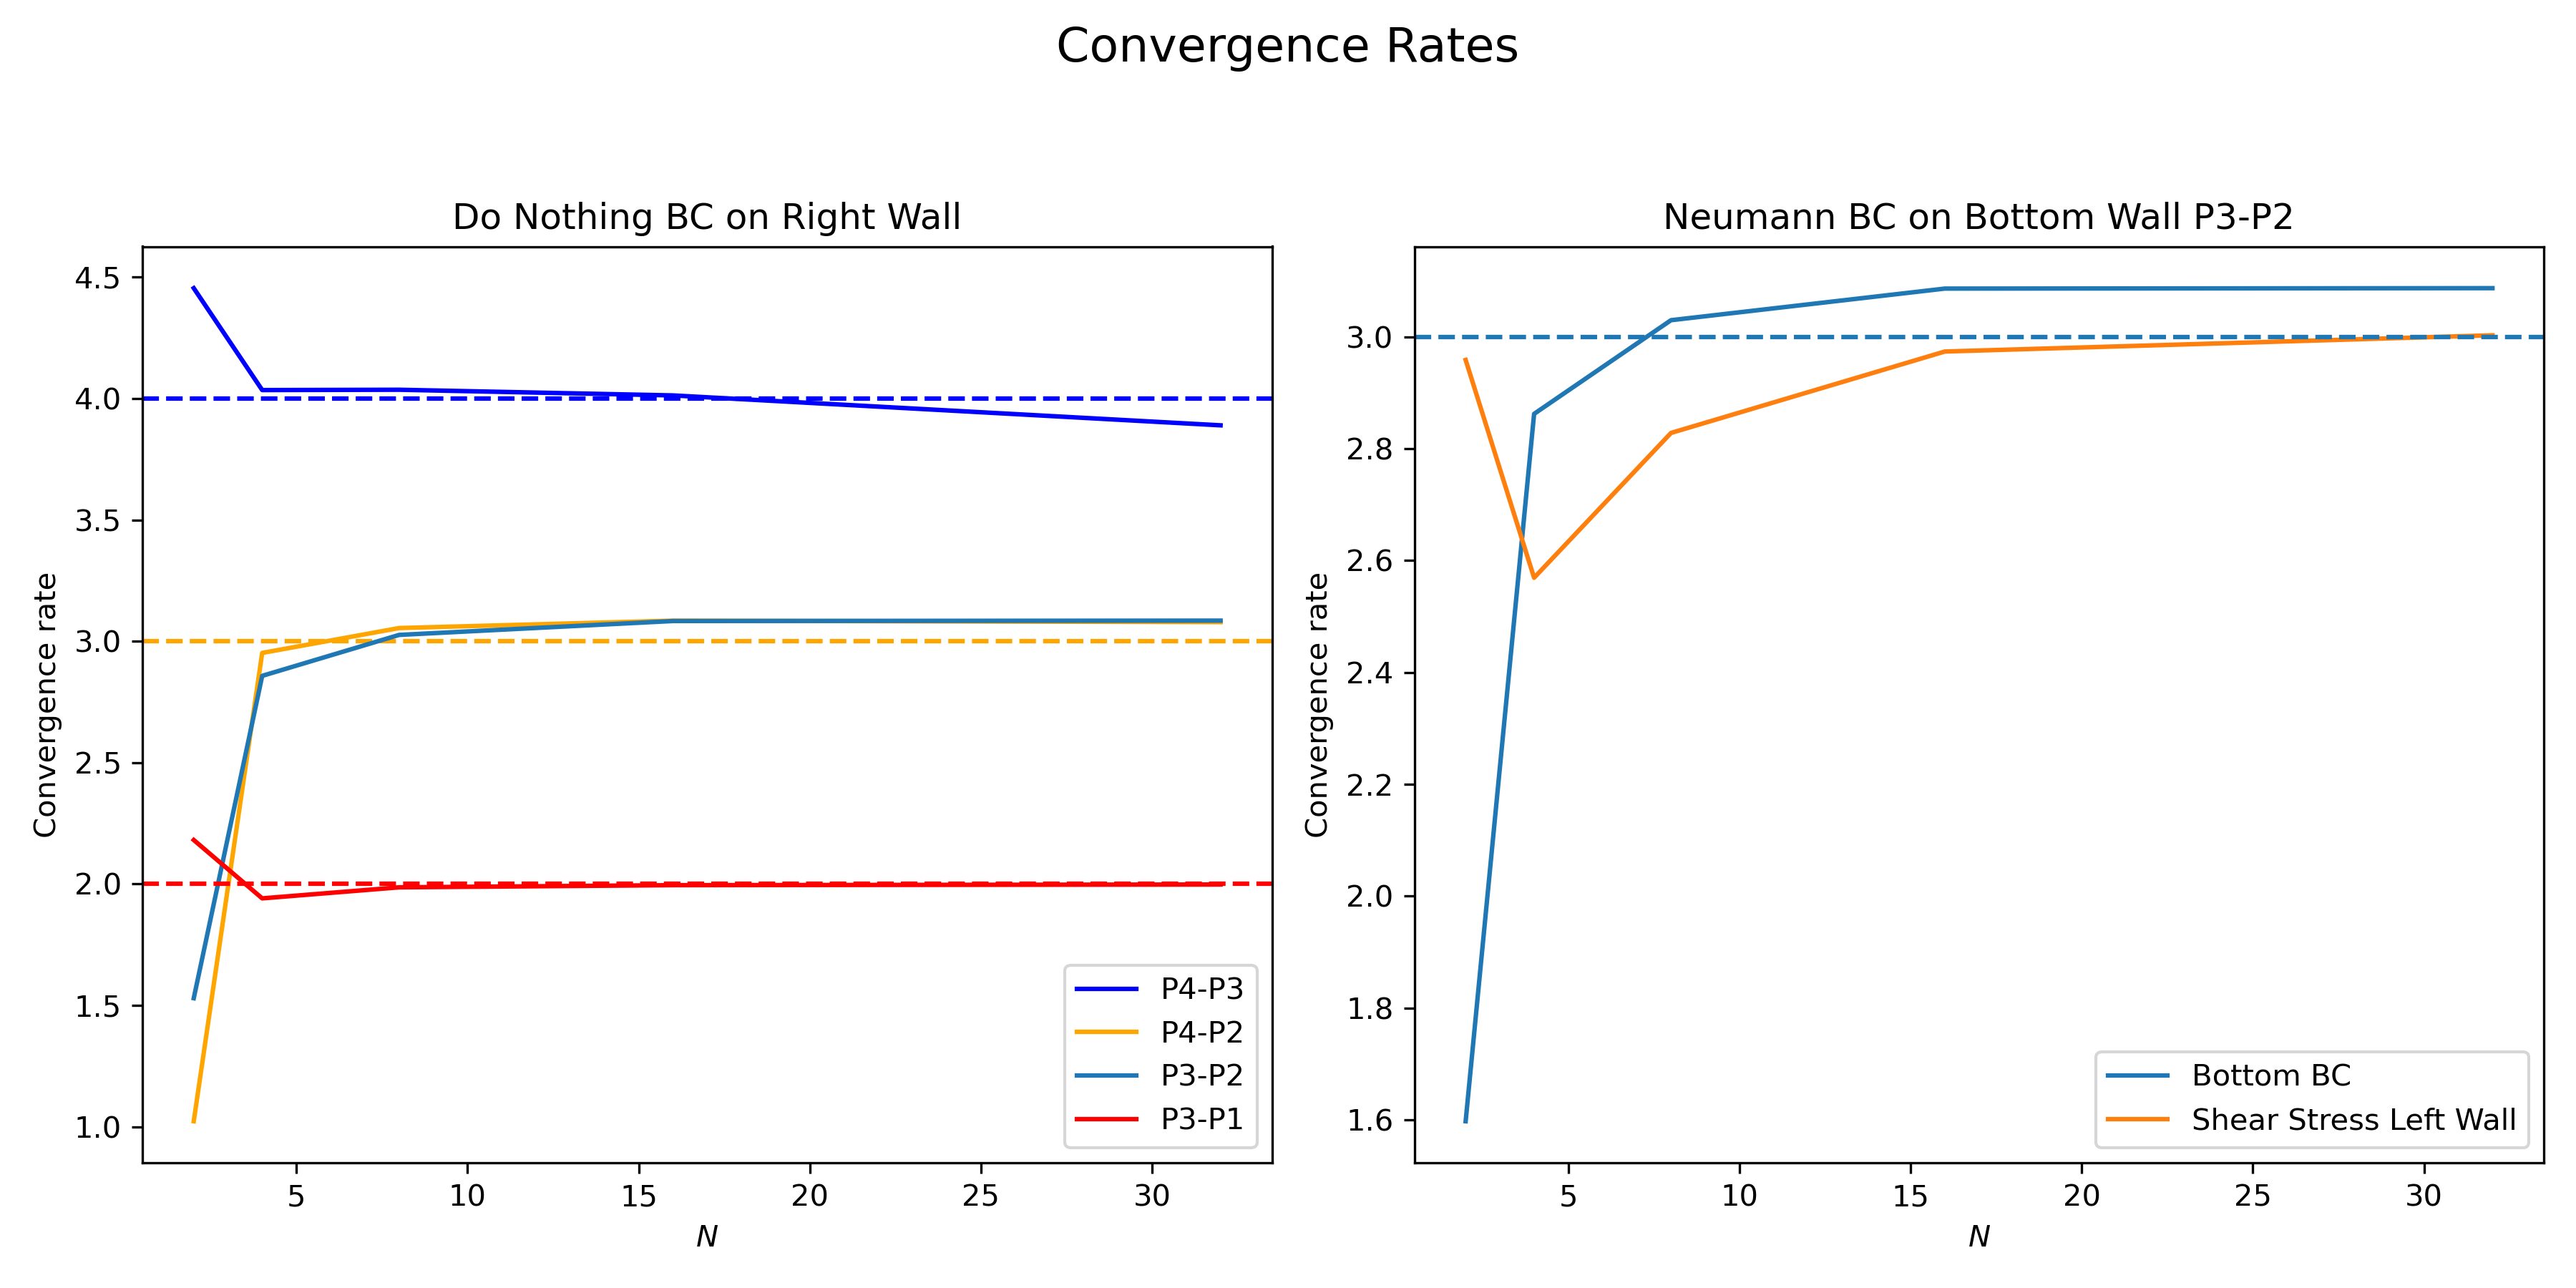
\includegraphics[width=1.1\linewidth]{figs/convergence_rates.png}
    \caption{Convergence for different element pairs. Dotted lines show expected convergence rates.}
    \label{fig:ex66}
\end{figure}

\begin{figure}[htbp]
    \centering
    % Subplot for Exercise 6.6
    \begin{subfigure}[t]{0.48\textwidth}
        \centering
        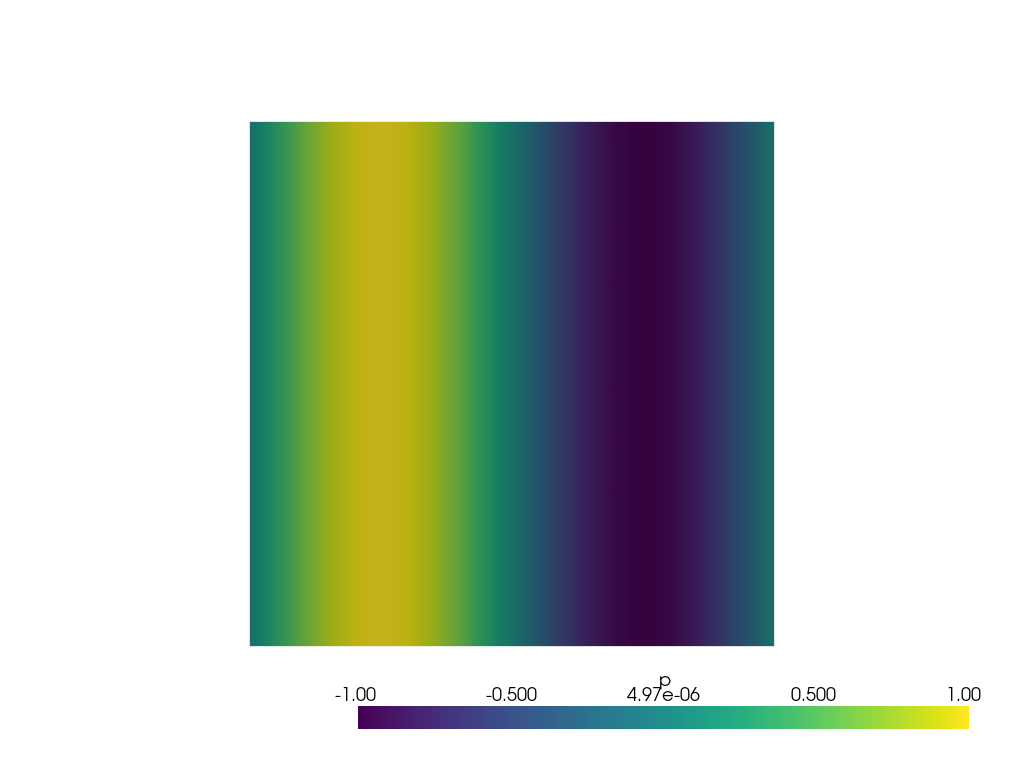
\includegraphics[width=\linewidth]{figs/pressure_66.png}
        \vspace{0.5em} % Optional spacing between images
        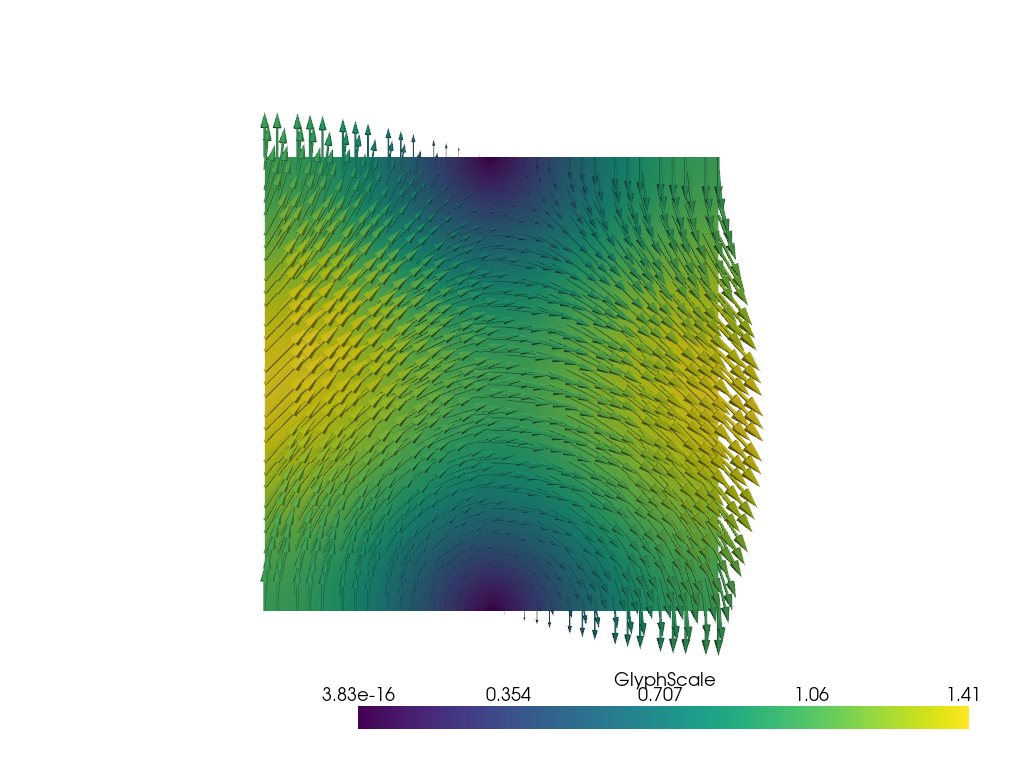
\includegraphics[width=\linewidth]{figs/velocity_66.png}
        \caption{Exercise 6.6: Pressure and Velocity}
        \label{fig:ex66}
    \end{subfigure}
    \hfill
    % Subplot for Exercise 6.7
    \begin{subfigure}[t]{0.48\textwidth}
        \centering
        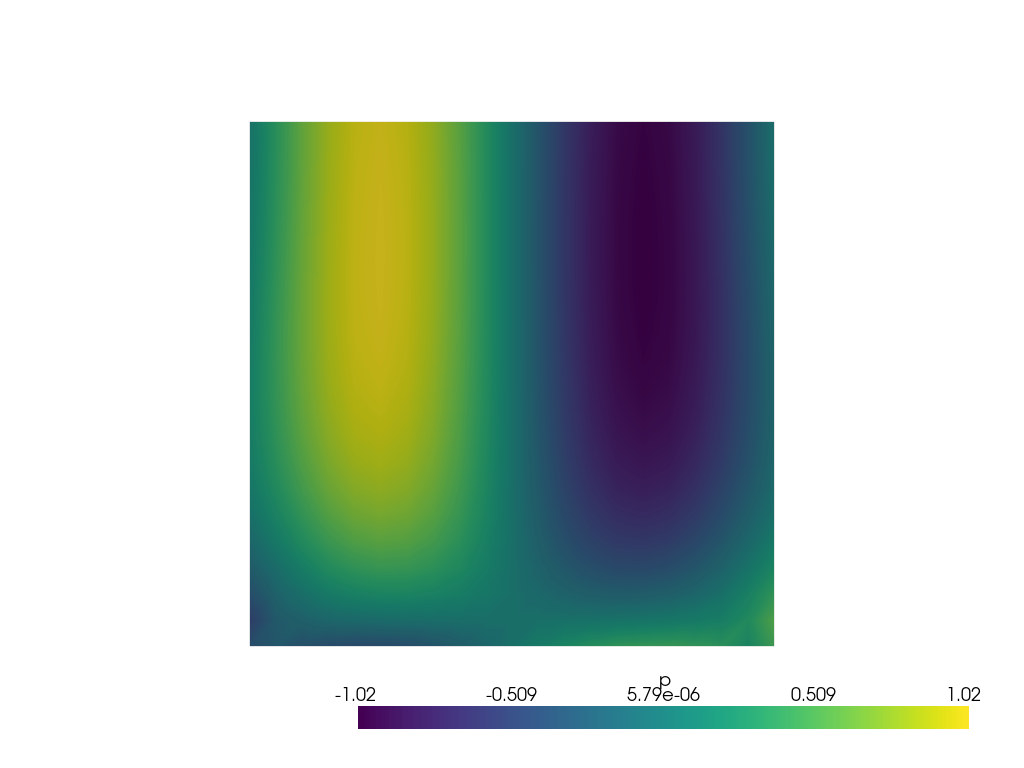
\includegraphics[width=\linewidth]{figs/pressure_67.png}
        \vspace{0.5em} % Optional spacing between images
        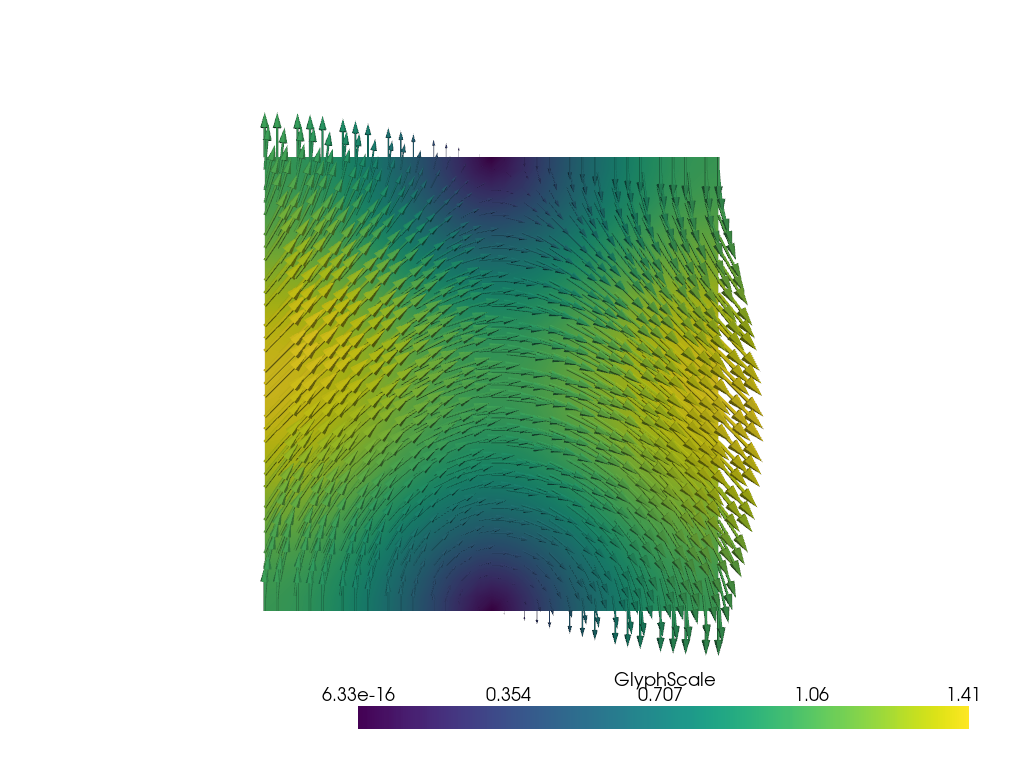
\includegraphics[width=\linewidth]{figs/velocity_67.png}
        \caption{Exercise 6.7: Pressure and Velocity}
        \label{fig:ex67}
    \end{subfigure}
    \caption{Pressure and Velocity Figures for Exercises 6.6 and 6.7.}
    \label{fig:combined}
\end{figure}


\FloatBarrier

Plotting

\inputminted[linenos, breaklines]{python}{plotter.py}






\end{document}